\subsection {An\'alisis de ECM y PSNR}

En el trabajo medimos la calidad de los m\'etodos para hacer una c\'amara lenta
de los videos bajando algunos videos con diferentes propiedades de internet
(osea que tienen relevancia en el mundo real), y sacando todos los frames
excepto uno de cada $c$. Luego se aplica alguno de los m\'etodos para generar un
video nuevo, con la misma cantidad de frames que el video original, que
idealmente ser\'ia igual (aunque es matem\'aticamente imposible \footnote{por el
principio del palomar} que haya un m\'etodo perfecto para todos los videos).

Luego, para medir el error entre el nuevo video en c\'amara lenta y el video
original se usa uno de dos m\'etodos: el \textbf{Error Cuadr\'atico Medio} o ECM
y el \textbf{Peak Signal to Nouse Ratio} o PSNR, que se definen como

\[
ECM(F, \bar{F}) = \frac{1}{m n} \sum^m_{i = i} \sum^n_{j = 1} \left| F_{k_{i j}} - \bar{F}_{k_{i j}} \right|^2
\]
\[
PSNR(F, \bar{F}) = 10 \; log_{10} \left( \frac{255^2}{ECM(F, \bar{F}} \right)
\]

Con $n$ igual a la altura de la im\'agen y $m$ igual a su largo. Estos dos
valores son importantes ya que, aunque los m\'etodos trabajen
``individualmente'' en un solo pixel, y el resultado de estos ser\'ian lo mismo
corriendose en mismo video que individualmente, ya que las pruebas son con videos
reales.

Hicimos los an\'alisis sobre 3 de los videos que contenian propiedades
interesantes: \textit{camerachanges.mp4}, \textit{slowmovescene.mp4}, y
\textit{funnybaby.avi}, y sobre los tres algoritmos. Como los videos son
relativamente peque\~nos y, por ende, el m\'etodo de splines es r\'apido,
dejamos el parametro $r$ del m\'etodo, que controla cada cuantos frames se
vuelven a empezar los splines, igual a $\infty$, osea que se hace un solo spline
para cada pixel del video.

Para ver como se comportaban los algoritmos mediante en salto, medimos el
\textbf{ECM} para saltos de 1, 3, 5, 7, y 10 frames:

\begin{figure}[H]
\centering
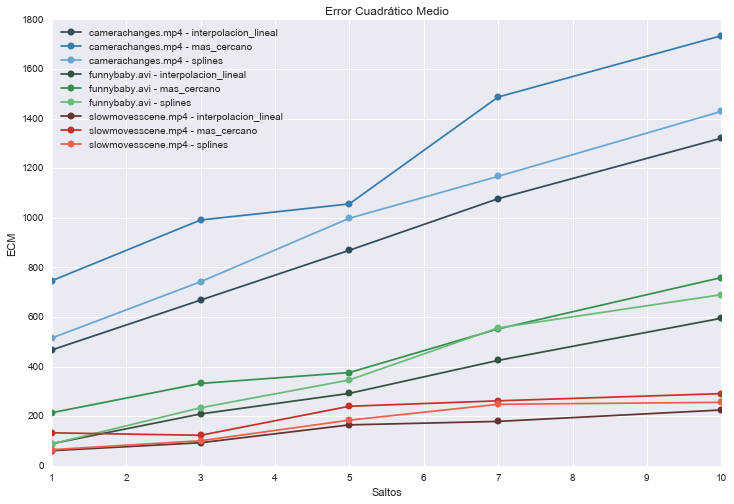
\includegraphics[width=.95\textwidth]{graficos/ecm.png}
\end{figure}

Este gr\'afico cementa la hipotesis de que \textit{camerachanges.avi}, que tiene
muchos cambios de c\'amara lo que hace que sea dificil predecir el valor de dos
pixeles cuando se pone en le c\'amara lenta tiene obviamente el mayor error. Por
otro lado, \textit{funnybaby.avi} y \textit{slowmoviescene.mp4} empiezan con un
\textbf{ECM} similar ya que ninguno de los dos tiene cambios bruscos, pero
cuando la cantidad de saltos aumenta el primer video empieza a tener un error
mucho mayor, ya que los cambios en el video dependientes del movimiento de la
cabeza del beb\'e \footnote{este es un beb\'e especialmente cabez\'on en comparaci\'on al
tama\~no del video} son mucho m\'as bruscos que los del video anterior.

Para comparar los m\'etodos, podemos ver el gr\'afico anterior y uno que tenga
solamente los valores para \textit{funnybaby.avi}

\begin{figure}[H]
\centering
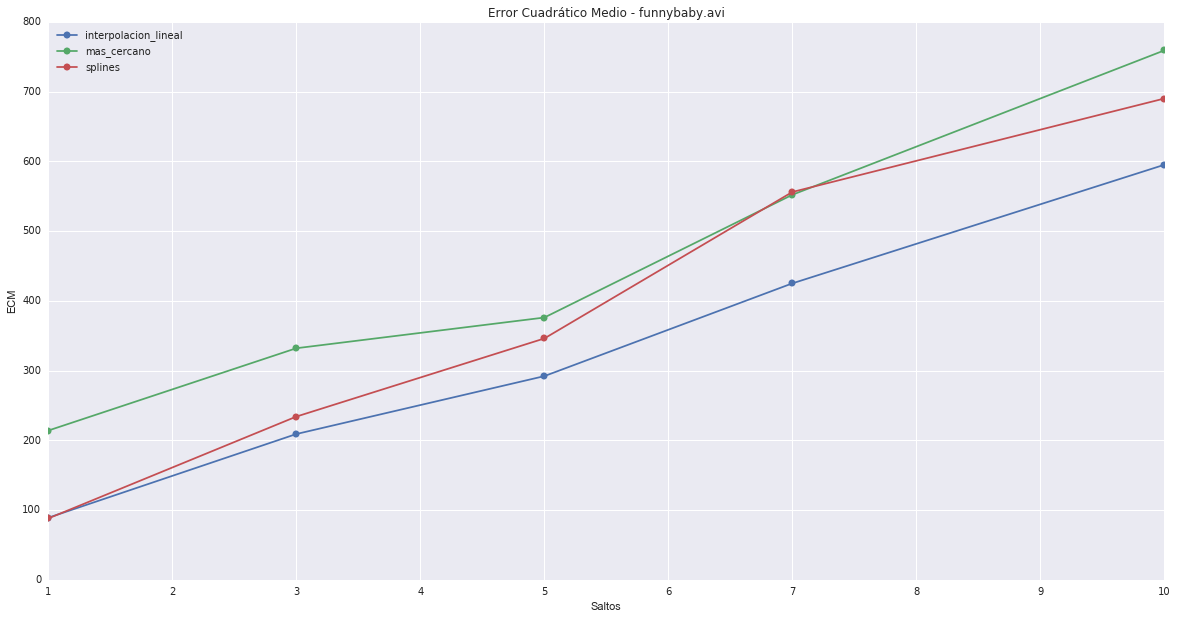
\includegraphics[width=.95\textwidth]{graficos/ecm_funnybaby.png}
\end{figure}

Como podemos ver, en todos los videos el m\'etodo de \textbf{interpolaci\'on
lineal} es el que genera menores errores, inclusive menos que el de splines.

El an\'alisis por \textbf{PSNR} da un resultado similar al de \textbf{ECM}, ya
que los dos m\'etodos est\'an inversamente relacionados. Sin embargo, se nota
con m\'as claridad que cuando hay pocos saltos el resultado puede ser altamente
diferente.

\begin{figure}[H]
\centering
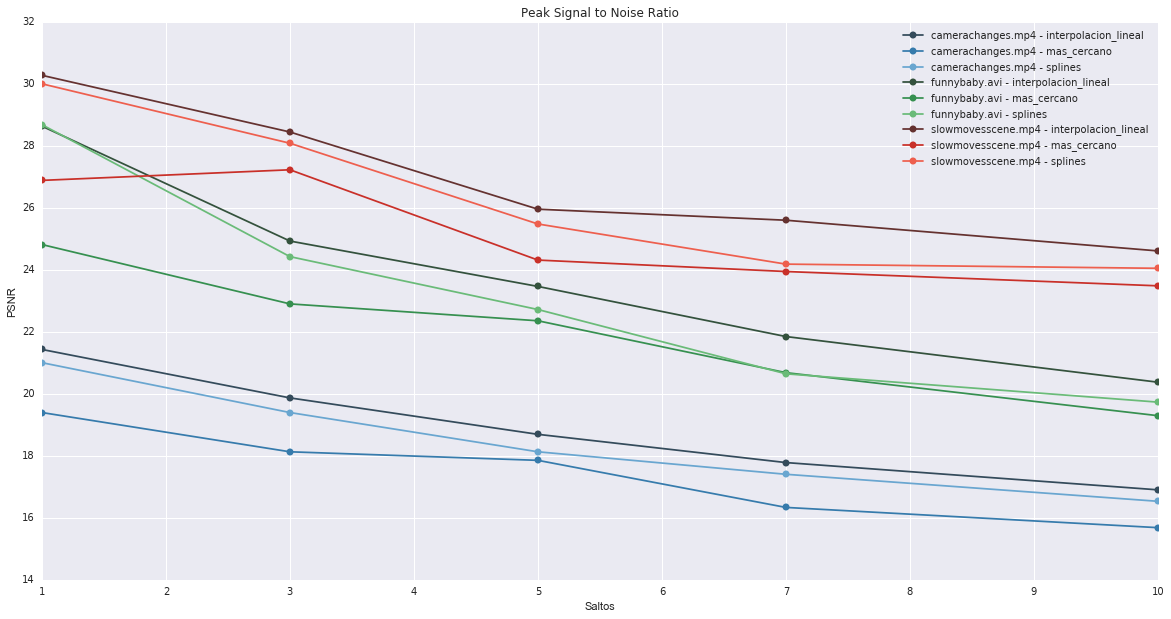
\includegraphics[width=.95\textwidth]{graficos/psnr.png}
\end{figure}

